\documentclass{article}

% Use final NeurIPS (two-column)
\usepackage[final]{neurips_2022}

% Basics
\usepackage[utf8]{inputenc}
\usepackage[T1]{fontenc}
\usepackage{microtype}
\usepackage{hyperref}
\usepackage{url}
\usepackage{amsmath,amssymb}
\usepackage{booktabs}
\usepackage{xcolor}
% Algorithm package - using algorithm2e for better compatibility
\usepackage[ruled,vlined,linesnumbered]{algorithm2e}


% Floats/graphics
\usepackage{caption}
\captionsetup{font=small}
\setlength{\textfloatsep}{6pt plus 2pt minus 2pt}
\setlength{\abovecaptionskip}{3pt}
\setlength{\belowcaptionskip}{0pt}

\usepackage{tikz}
\usetikzlibrary{positioning,arrows.meta}

\title{Project Milestone --- Literature Review:\\ A Dual--SPMA Framework for Convex MDPs}

\author{
Shervin Khamooshian \quad Ahmed Magd \quad Pegah Aryadoost \quad Danielle Nguyen\\
Simon Fraser University \qquad \texttt{\{ska309, ams80, paa40, tdn8\}@sfu.ca}
}

\begin{document}
\maketitle

% ============================================================================
% SECTION 1: PROJECT TOPIC
% ============================================================================

\section{Project Topic}

\textbf{Goal.} We study a unified way to solve \emph{Convex MDPs (CMDPs)} by combining a Fenchel-dual saddle formulation with a geometry-aware policy optimizer, \emph{Softmax Policy Mirror Ascent (SPMA)}. CMDPs minimize a convex function of discounted occupancies and are equivalent to the saddle
$\min_{\pi}\max_{y}\ \langle y,d_{\pi}\rangle-f^*(y)$. Fixing $y$ turns the policy step into standard RL with shaped reward $r_y(s,a)=-y(s,a)$ (or $-\,\phi(s,a)^\top y$ under features). We alternate a mirror-ascent step on $y$ with an SPMA policy step and return discounted occupancy (or feature-expectation) estimates for the next dual update (Fig.~\ref{fig:dualspma}).

\begin{figure}[htbp]
\centering
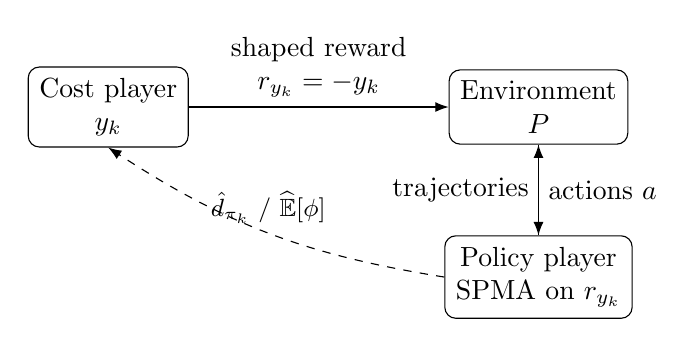
\begin{tikzpicture}[node distance=1.55cm, >=Latex]
\node[draw, rounded corners, align=center, inner sep=4pt] (cost) {Cost player\\$y_k$};
\node[draw, rounded corners, align=center, inner sep=4pt, right=3.3cm of cost] (env) {Environment\\$P$};
\node[draw, rounded corners, align=center, inner sep=4pt, below=1.15cm of env] (policy) {Policy player\\SPMA on $r_{y_k}$};
\draw[->] (cost) -- node[above, align=center]{shaped reward\\$r_{y_k}=-y_k$} (env);
\draw[->] (policy) -- node[right]{actions $a$} (env);
\draw[->] (env) -- node[left]{trajectories} (policy);
\draw[->, dashed, bend left=12] (policy.west) to node[above]{\small $\hat d_{\pi_k}$ / $\widehat{\mathbb E}[\phi]$} (cost.south);
\end{tikzpicture}
\caption{\textbf{Dual--SPMA loop.} Dual ascent chooses $y_k$, which induces a shaped reward for the SPMA policy step; discounted occupancies feed the next dual update.}
\label{fig:dualspma}
\end{figure}


% ============================================================================
% SECTION 2: LITERATURE REVIEW - PAPER SUMMARIES
% ============================================================================
\section{Literature Review: Paper Summaries}

We review three foundational papers that inform our Dual--SPMA framework: (1) the Fenchel duality approach for convex MDPs, (2) the SPMA policy optimizer with fast convergence, and (3) primal-dual methods for constrained MDPs.


% ──────────────────────────────────────────────────────────────────────────
\subsection{Paper 1: \emph{Reward is Enough for Convex MDPs} (NeurIPS 2021)}
\textbf{Core idea.} Many RL goals can be posed as $\min_{d\in\mathcal{K}} f(d)$ for convex $f$ over the occupancy polytope $\mathcal{K}$. Using Fenchel conjugacy,
\(
\min_{d\in \mathcal{K}} f(d)=\min_{d\in \mathcal{K}}\max_{\lambda\in\Lambda}\ \lambda\!\cdot\! d - f^*(\lambda),
\)
so for fixed $\lambda$ the policy subproblem is vanilla RL with shaped reward $r_\lambda=-\lambda$. 

\begin{figure}[htbp]
\centering
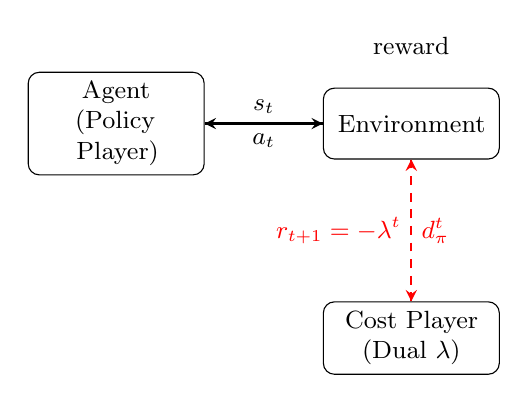
\begin{tikzpicture}[
    node distance=1.5cm,
    block/.style={rectangle, draw, text width=2cm, text centered, 
                  minimum height=0.9cm, rounded corners, font=\small},
    arrow/.style={->, >=stealth, thick}
]
\node[block] (agent) {Agent\\(Policy Player)};
\node[block, right=of agent] (env) {Environment};
\node[block, below=1.8cm of env] (cost) {Cost Player\\(Dual $\lambda$)};
\draw[arrow] (env) -- node[above, font=\small] {$s_t$} (agent);
\draw[arrow] (agent) -- node[below, font=\small] {$a_t$} (env);
\draw[arrow, dashed, red, thick] (cost) -- node[left, font=\small] {$r_{t+1} = -\lambda^t$} (env);
\draw[arrow, dashed, red, thick] (env) -- node[right, font=\small] {$d_\pi^t$} (cost);
\node[above=0.3cm of env, font=\small] {reward};
\end{tikzpicture}
\caption{Convex MDP as a two-player game (adapted from \citet{zahavy2021reward}, Fig.~1). 
The cost player provides non-stationary shaped rewards $r_t = -\lambda^t$ to the agent, 
observing the resulting occupancy measures $d_\pi^t$. From the agent's perspective, this 
reduces to standard RL with time-varying rewards.}
\label{fig:convex_mdp_game}
\end{figure}

Figure~\ref{fig:convex_mdp_game} illustrates this as a two-player game where the agent sees non-stationary rewards from the cost player. A meta-algorithm (Algorithm~\ref{alg:convex_mdp_meta}) alternates a \emph{cost player} (FTL/OMD in $\lambda$, a convex ascent step) with a \emph{policy player} (best response or low-regret RL, which reduces to ``just RL'' under the shaped reward), yielding $O(1/\sqrt{K})$ optimization error for averaged iterates under standard OCO assumptions. The paper shows best-response is ideal but often intractable in deep RL, so low-regret learners (e.g., UCRL2, MDPO) suffice; the guarantees hold for averaged occupancies $\bar{d}_\pi^K$ rather than single iterates. It unifies apprenticeship learning, CMDPs and pure exploration (Table~\ref{tab:convex_mdp_examples}). \citep{zahavy2021reward}

% Algorithm using algorithm2e syntax
\begin{algorithm}[htbp]
\caption{Meta-algorithm for Convex MDPs \citep{zahavy2021reward}}
\label{alg:convex_mdp_meta}
\small
\KwIn{Convex-concave payoff $\mathcal{L}: \mathcal{K} \times \Lambda \to \mathbb{R}$, algorithms $\text{Alg}_\lambda$, $\text{Alg}_\pi$, $K \in \mathbb{N}$}
\For{$k = 1, \ldots, K$}{
    $\lambda^k \leftarrow \text{Alg}_\lambda(d_\pi^1, \ldots, d_\pi^{k-1}; \mathcal{L})$ \tcp*{Cost player update}
    $d_\pi^k \leftarrow \text{Alg}_\pi(-\lambda^k)$ \tcp*{Policy: solve RL with $r = -\lambda^k$}
}
\KwOut{$\bar{d}_\pi^K = \frac{1}{K}\sum_{k=1}^K d_\pi^k$, $\bar{\lambda}^K = \frac{1}{K}\sum_{k=1}^K \lambda^k$}
\end{algorithm}

\begin{table}[htbp]
\centering
\caption{Instantiations of the convex MDP framework (adapted from \citet{zahavy2021reward}, Table~1). Different choices of objective $f$ and player algorithms recover well-known RL problems.}
\label{tab:convex_mdp_examples}
\small
\begin{tabular}{@{}p{3.5cm}p{4cm}p{3cm}p{3.5cm}@{}}
\toprule
\textbf{Application} & \textbf{Objective $f(d_\pi)$} & \textbf{Cost Player} & \textbf{Policy Player} \\
\midrule
Standard RL & $-\lambda \cdot d_\pi$ (linear) & FTL & RL \\
Apprenticeship Learning & $\|d_\pi - d_E\|_2^2$ & FTL & Best Response \\
Pure Exploration & $d_\pi \cdot \log(d_\pi)$ (entropy) & FTL & Best Response \\
AL with $\ell_\infty$ & $\|d_\pi - d_E\|_\infty$ & OMD & Best Response \\
Constrained MDPs & $\lambda_1 \cdot d_\pi$ s.t. $\lambda_2 \cdot d_\pi \leq c$ & OMD & RL \\
GAIL / State Matching & $\text{KL}(d_\pi \| d_E)$ & FTL & RL \\
\bottomrule
\end{tabular}
\end{table}


\textbf{Relevance.} This work justifies the saddle and the shaped-reward reduction we implement and informs our outer-loop design (dual MA + policy best response).

% ──────────────────────────────────────────────────────────────────────────
\subsection{Paper 2: \emph{Fast Convergence of Softmax Policy Mirror Ascent} (OPT 2024 / arXiv 2025)}

\textbf{Core idea.} \emph{SPMA} performs mirror ascent in \emph{logit} space using the log-sum-exp mirror map. In tabular MDPs the per-state update
$\pi_{t+1}(a|s)=\pi_t(a|s)\bigl(1+\eta\,A^{\pi_t}(s,a)\bigr)$
avoids explicit normalization and achieves \emph{linear convergence} for sufficiently small constant step-size, improving over softmax PG. For large problems, SPMA projects onto function classes via convex \emph{softmax classification} subproblems and proves linear convergence to a neighbourhood under FA; empirically it competes with PPO/TRPO/MDPO. \citep{asad2024fast}

\textbf{Relevance.} We need a strong policy ``best response'' in Zahavy's saddle; SPMA provides the geometry and rates, and its FA projection matches our shaped-reward reduction.

% ──────────────────────────────────────────────────────────────────────────

\subsection{Paper 3: \emph{Natural Policy Gradient Primal--Dual for CMDPs} (NeurIPS 2020)}
\textbf{Core idea.} A policy-based primal--dual method: \emph{natural policy gradient} (NPG) ascent for the policy and projected subgradient updates for the multiplier. Despite nonconcavity/nonconvexity under softmax parameterization, it proves \emph{dimension-free} $O(1/\sqrt{T})$ bounds on averaged optimality gap and constraint violation; with FA, rates hold up to an approximation neighbourhood; sample-based variants have finite-sample guarantees. \citep{ding2020npgpd}

\textbf{Relevance.} NPG--PD is our principled CMDP baseline for both guarantees and practice; we compare Dual--SPMA against it in convergence/violation/sample-efficiency.

% ============================================================================
% SECTION 3: HOW THE PAPERS RELATE TO EACH OTHER
% ============================================================================

\section{How the Papers Relate to Each Other and to our project}

The three papers provide complementary perspectives on our Dual--SPMA framework (Fig.~\ref{fig:framework_overview}):

\textbf{Formulation.} Zahavy et~al.\ provide the \emph{outer-loop template}: the Fenchel-dual saddle formulation that reduces constrained/structured RL to alternating between a cost player (dual ascent) and a policy player (shaped-reward RL). This formulation is key because fixing the dual variable $y$ yields standard RL with shaped reward $r_y = -y$.

\textbf{Policy player.} SPMA (Asad et~al.) supplies the \emph{fast policy player} for the RL step in Zahavy's framework. It performs mirror ascent in logit space, achieving linear convergence rates in tabular settings and practical function approximation via convex softmax classification. This makes SPMA an ideal candidate for the policy subproblem.

\textbf{Baseline and dual updates.} NPG--PD (Ding et~al.) offers a \emph{policy-based CMDP baseline} with dimension-free sublinear guarantees. While we use SPMA (not NPG) as our policy player, Ding et~al.\ inform how we handle constraint multipliers via projected subgradient updates and serve as our principled comparison baseline.

Table~\ref{tab:comparison} summarizes how these three approaches differ in their formulation, policy optimization method, and convergence guarantees.

% FIXED TABLE - using proper p{} columns instead of tabularx
\begin{table}[htbp]
\caption{Three perspectives that our project unifies or compares against.}
\label{tab:comparison}
\centering
\small
\setlength{\tabcolsep}{3pt}
\begin{tabular}{@{}p{2.8cm}p{3.8cm}p{2.8cm}p{3.8cm}@{}}
\toprule
\textbf{Work} & \textbf{Objective / Saddle} & \textbf{Policy Player} & \textbf{Guarantees / Notes} \\
\midrule
Zahavy et al.\ (2021) \citep{zahavy2021reward} & $\min_{d} f(d)$; Fenchel dual $\min_d \max_\lambda \lambda\!\cdot\! d - f^{*}(\lambda)$ & Best response / low-regret RL under $r_\lambda=-\lambda$ & $O(1/\sqrt{K})$ via OCO; unifies AL, CMDPs, exploration \\[6pt]
Asad et al.\ (2025) \citep{asad2024fast} & RL inner step (fixed $y$) & SPMA: $\pi_{t+1}=\pi_t(1+\eta A)$; FA via convex projection & Linear (tabular); neighbourhood (FA); strong empirical results \\[6pt]
Ding et al.\ (2020) \citep{ding2020npgpd} & Lagrangian CMDP $\max_\pi \min_{\lambda\ge0} V_r^\pi+\lambda(V_g^\pi-b)$ & NPG for $\pi$, projected subgradient for $\lambda$ & Dimension-free $O(1/\sqrt{T})$ gap \& violation (avg.) \\
\bottomrule
\end{tabular}
\end{table}

% Overview picture of how everything fits together
\begin{figure}[htbp]
\centering
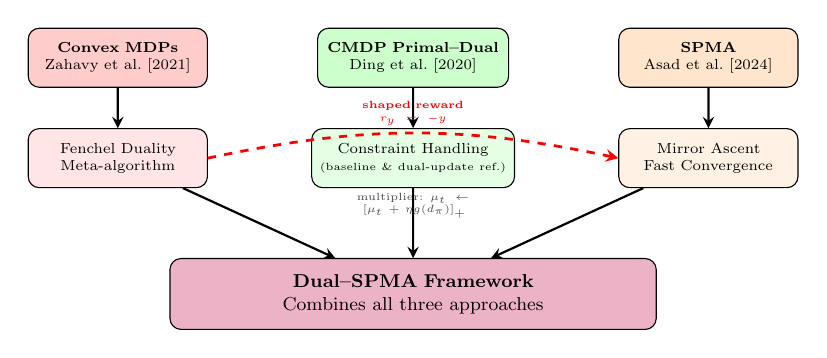
\begin{tikzpicture}[
    block/.style={rectangle, draw, text width=2.8cm, text centered, rounded corners, minimum height=1cm, font=\scriptsize},
    arrow/.style={->, >=stealth, thick},
    scale=0.75, transform shape
]

% Top row: Three source papers
\node[block, fill=red!20] (paper1) at (0,4.5) {
    \textbf{Convex MDPs}\\
    Zahavy et al.\ [2021]
};
\node[block, fill=green!20, text width=3cm] (paper2) at (5,4.5) {
    \textbf{CMDP Primal--Dual}\\
    Ding et al.\ [2020]
};
\node[block, fill=orange!20] (paper3) at (10,4.5) {
    \textbf{SPMA}\\
    Asad et al.\ [2024]
};

% Middle row: Contributions
\node[block, fill=red!10] (contrib1) at (0,2.8) {
    Fenchel Duality\\
    Meta-algorithm
};
\node[block, fill=green!10, text width=3.2cm] (contrib2) at (5,2.8) {
    Constraint Handling\\
    {\tiny (baseline \& dual-update ref.)}
};
\node[block, fill=orange!10] (contrib3) at (10,2.8) {
    Mirror Ascent\\
    Fast Convergence
};

% Multiplier note
\node[font=\tiny, text width=3cm, align=center, text=black!70] at (5,2) {
    multiplier: $\mu_t \leftarrow [\mu_t + \eta g(d_\pi)]_+$
};

% Bottom: Our framework
\node[block, fill=purple!30, text width=8cm, minimum height=1.2cm, font=\small] (ours) at (5,0.5) {
    \textbf{Dual--SPMA Framework}\\
    Combines all three approaches
};

% Vertical arrows
\draw[arrow] (paper1) -- (contrib1);
\draw[arrow] (paper2) -- (contrib2);
\draw[arrow] (paper3) -- (contrib3);

% Key connection arrow
\draw[arrow, dashed, red, bend left=12, line width=1pt] (contrib1.east) to 
    node[above, font=\tiny, text width=2.5cm, align=center] {
        \textbf{shaped reward}\\
        $r_y = -y$
    } (contrib3.west);

% Arrows to framework
\draw[arrow] (contrib1) -- (ours);
\draw[arrow] (contrib2) -- (ours);
\draw[arrow] (contrib3) -- (ours);

\end{tikzpicture}
\caption{Overview of how the three papers inform our Dual--SPMA framework. The key insight is that Zahavy's shaped reward reduction ($r_y = -y$) enables us to use SPMA as the policy player, while Ding et al.\ inform our constraint handling and serve as a baseline.}
\label{fig:framework_overview}
\end{figure}


\section{What we will implement and measure}
\textbf{Method.} Dual--SPMA: $y_{k+1}\!\leftarrow\!\mathrm{MA}\!\left(y_k,\,\hat d_{\pi_k}-\nabla f^*(y_k)\right)$; policy step: run SPMA for $K_{\text{in}}$ epochs on $r_{y_k}$; return $\hat d_{\pi_k}$ (or $\widehat{\mathbb E}[\phi]$).

\textbf{Metrics.} (i) Saddle value $L(\pi,y)$ (when $f^*$ known); (ii) constraint value/violation; (iii) policy return under $r_y$; (iv) convergence of $\|\hat d_{\pi}\|_1$ (tabular) or $\|\widehat{\mathbb E}[\phi]\|$ (FA); (v) wall-clock/sample efficiency. Baselines include NPG--PD.

\small
\bibliographystyle{abbrvnat}
\bibliography{refs}

\appendix

\section{Discounted Occupancy Measures and Feature Expectations}

This appendix provides formal definitions and estimation procedures for the discounted occupancy measure $\hat{d}_\pi$ and feature expectations $\widehat{\mathbb{E}}[\phi]$ that appear in our Dual--SPMA framework (Fig.~\ref{fig:dualspma}).

% ────────────────────────────────────────────────────
\subsection{Discounted Occupancy Measure (Tabular Setting)}

\paragraph{Definition.}
For a policy $\pi$ in an MDP with discount factor $\gamma \in [0,1)$ and initial state distribution $\rho$, the \textbf{discounted occupancy measure} is defined as:
\[
d_\pi(s,a) = (1-\gamma) \sum_{t=0}^{\infty} \gamma^t \Pr(s_t=s, a_t=a \mid \pi, \rho).
\]
This quantity represents the discounted frequency with which policy $\pi$ visits state-action pair $(s,a)$. The normalization factor $(1-\gamma)$ ensures that $\sum_{s,a} d_\pi(s,a) = 1$, making $d_\pi$ a valid probability distribution over $\mathcal{S} \times \mathcal{A}$.

\paragraph{Properties.}
The occupancy measure uniquely characterizes a policy and satisfies:
\begin{itemize}
    \item \textbf{Linearity of rewards:} The expected return can be expressed as $V_r^\pi(\rho) = \sum_{s,a} d_\pi(s,a) \, r(s,a) = \langle d_\pi, r \rangle$.
    \item \textbf{Polytope structure:} The set of all valid occupancy measures forms a convex polytope $K \subseteq \mathbb{R}^{|\mathcal{S}| \times |\mathcal{A}|}$, enabling convex optimization over policies.
\end{itemize}

\paragraph{Estimation.}
In practice, we estimate $d_\pi$ from sampled trajectories. Given $N$ trajectories of horizon $H$, the empirical estimate is:
\[
\hat{d}_\pi(s,a) = \frac{1}{N} \sum_{i=1}^{N} \sum_{t=0}^{H-1} \gamma^t \, \mathbb{I}[s_t^{(i)}=s, a_t^{(i)}=a] \cdot \frac{(1-\gamma)}{1-\gamma^H},
\]
where $\mathbb{I}[\cdot]$ is the indicator function and the normalization factor $(1-\gamma)/(1-\gamma^H)$ accounts for the finite horizon.

% ────────────────────────────────────────────────────
\subsection{Feature Expectations (Function Approximation Setting)}

\paragraph{Motivation.}
In large or continuous state-action spaces (e.g., robotics, Atari), tracking the full occupancy measure $d_\pi(s,a)$ becomes intractable due to the curse of dimensionality. Instead, we represent the occupancy through a finite-dimensional \textbf{feature map} $\phi: \mathcal{S} \times \mathcal{A} \to \mathbb{R}^d$, where $d \ll |\mathcal{S}| \times |\mathcal{A}|$.

\paragraph{Definition.}
The \textbf{feature expectation} under policy $\pi$ is:
\[
\mathbb{E}_{d_\pi}[\phi] = \sum_{s,a} d_\pi(s,a) \, \phi(s,a) \in \mathbb{R}^d.
\]
This is a $d$-dimensional vector that summarizes the policy's occupancy distribution in feature space.

\paragraph{Shaped Reward under Features.}
In the Fenchel dual formulation with features, the dual variable becomes $y \in \mathbb{R}^d$ (instead of $y \in \mathbb{R}^{|\mathcal{S}| \times |\mathcal{A}|}$), and the shaped reward is:
\[
r_y(s,a) = -\phi(s,a)^\top y.
\]
The saddle-point problem becomes:
\[
\min_{\pi} \max_{y \in \mathbb{R}^d} \langle y, \mathbb{E}_{d_\pi}[\phi] \rangle - f^*(y).
\]

\paragraph{Estimation.}
Given $N$ sampled trajectories, we estimate the feature expectation as:
\[
\widehat{\mathbb{E}}[\phi] = \frac{1}{N} \sum_{i=1}^{N} \sum_{t=0}^{H-1} \gamma^t \, \phi(s_t^{(i)}, a_t^{(i)}) \cdot \frac{(1-\gamma)}{1-\gamma^H}.
\]
This reduces the communication between the policy player and cost player from $|\mathcal{S}| \times |\mathcal{A}|$ dimensions to just $d$ dimensions, making the algorithm scalable.

% ────────────────────────────────────────────────────
\subsection{Role in the Dual--SPMA Algorithm}

% \begin{algorithm}[htbp]
% \caption{Dual-SPMA for Convex CMDPs}
% \label{alg:dual_spma}
% \begin{algorithmic}[1]
% \STATE \textbf{Input:} Initial policy $\pi_0$ (uniform), step-sizes $\eta_1, \eta_2$, iterations $T$
% \STATE \textbf{Initialize:} $\theta^0 = \mathbf{0}$, $\lambda^0 = \mathbf{0}$, $\mu^0 = \mathbf{0}$
% \FOR{$t = 0, 1, \ldots, T-1$}
%     \STATE \textbf{// Cost player update (dual)}
%     \STATE Compute gradient: $\nabla f(d_{\pi_t})$ and constraint violations $g_i(d_{\pi_t})$
%     \STATE Update dual variables:
%     \STATE \quad $\lambda^{t+1} = \lambda^t + \eta_2 \nabla f(d_{\pi_t})$
%     \STATE \quad $\mu_i^{t+1} = [\mu_i^t - \eta_2 g_i(d_{\pi_t})]_+$ for $i=1,\ldots,m$
%     \STATE 
%     \STATE \textbf{// Policy player update (primal - SPMA)}
%     \STATE Form composite cost: $\tilde{\lambda}^{t+1} = \lambda^{t+1} + \sum_{i=1}^m \mu_i^{t+1} \nabla g_i(d_{\pi_t})$
%     \STATE Compute advantages: $A^{\pi_t}(s,a) = Q^{\pi_t}(s,a) - V^{\pi_t}(s)$ w.r.t. $\tilde{\lambda}^{t+1}$
%     \STATE \textbf{// SPMA update (no normalization needed)}
%     \STATE $\pi_{t+1}(a|s) = \pi_t(a|s) \cdot (1 + \eta_1 A^{\pi_t}(s,a))$ for all $s,a$
% \ENDFOR
% \STATE \textbf{Return:} $\bar{\pi}^T = \frac{1}{T}\sum_{t=0}^{T-1} \pi^t$ (averaged policy)
% \end{algorithmic}
% \end{algorithm}


In our framework (Algorithm~\ref{alg:dual-spma}, Fig.~\ref{fig:dualspma}), at each iteration $k$:

\begin{enumerate}
    \item The \textbf{cost player} provides a dual variable $y_k$ that defines the shaped reward:
    \[
    r_{y_k}(s,a) = 
    \begin{cases}
    -y_k(s,a) & \text{(tabular)} \\
    -\phi(s,a)^\top y_k & \text{(function approximation)}
    \end{cases}
    \]
    
    \item The \textbf{policy player} runs SPMA with reward $r_{y_k}$ to obtain policy $\pi_k$.
    
    \item We estimate the occupancy from sampled trajectories:
    \[
    \text{Estimate } = 
    \begin{cases}
    \hat{d}_{\pi_k}(s,a) & \text{(tabular)} \\
    \widehat{\mathbb{E}}_{d_{\pi_k}}[\phi] & \text{(function approximation)}
    \end{cases}
    \]
    
    \item This estimate is fed back to the cost player for the next dual update:
    \[
    y_{k+1} \leftarrow \text{MirrorAscent}\big(y_k, \hat{d}_{\pi_k} - \nabla f^*(y_k)\big).
    \]
\end{enumerate}

\paragraph{Example: Apprenticeship Learning.}
In imitation learning, we have an expert policy with occupancy $d_E$ (or feature expectation $\mathbb{E}_{d_E}[\phi]$). The objective is to minimize $f(d_\pi) = \|d_\pi - d_E\|_2^2$. The dual variable $y_k$ adjusts to penalize deviations from the expert's behavior, and the policy player learns by maximizing the shaped reward $r_{y_k}$.

\paragraph{Computational Complexity.}
\begin{itemize}
    \item \textbf{Tabular:} $\mathcal{O}(|\mathcal{S}| \times |\mathcal{A}|)$ storage and communication per iteration.
    \item \textbf{Function approximation:} $\mathcal{O}(d)$ storage and communication, enabling scalability to large domains.
\end{itemize}

% Optional: Add example
\subsection{Numerical Example}

Consider a simple $2$-state, $2$-action MDP with $\gamma=0.9$ and uniform initial distribution. Suppose we run policy $\pi$ and observe:
\begin{itemize}
    \item State-action $(s_1, a_1)$ visited at times $t=0, 2, 4$ in one trajectory
    \item State-action $(s_1, a_2)$ visited at time $t=1$ in one trajectory
\end{itemize}

The empirical occupancy estimate (for a single trajectory with $H=5$) would be:
\[
\hat{d}_\pi(s_1, a_1) \approx (1-\gamma) \cdot \frac{\gamma^0 + \gamma^2 + \gamma^4}{1-\gamma^5} = 0.1 \cdot \frac{1 + 0.81 + 0.6561}{0.40951} \approx 0.601
\]

In the feature approximation case with $\phi(s_1,a_1) = [1, 0]^\top$ and $\phi(s_1,a_2) = [0, 1]^\top$, we would compute:
\[
\widehat{\mathbb{E}}[\phi] \approx (1-\gamma) \cdot \frac{[1,0] \cdot \gamma^0 + [0,1] \cdot \gamma^1 + [1,0] \cdot \gamma^2 + [1,0] \cdot \gamma^4}{1-\gamma^5}.
\]
% ------------------------------------
\section*{Appendix A: What Figure~\ref{fig:dualspma} Shows and Where It Comes From}

\subsection*{A.1 Notation and objects in the diagram}
\begin{itemize}
\item $\pi(a|s)$: stochastic policy; $\gamma\in(0,1)$: discount.
\item \textbf{Discounted occupancy} of $(s,a)$ under $\pi$:
$d_\pi(s,a)=(1-\gamma)\sum_{t\ge0}\gamma^t\,\Pr_\pi(s_t=s,a_t=a)$.
\item $f:\mathbb{R}^{|\mathcal{S}\times\mathcal{A}|}\to\mathbb{R}$: convex objective on occupancies (task-specific).
\item $f^*$: Fenchel conjugate of $f$; $\langle u,v\rangle=\sum_{s,a} u(s,a)v(s,a)$.
\item \textbf{Dual/cost variable} $y$ (same dimension as costs or feature weights).
\item \textbf{Environment} $P$: transition kernel; emits trajectories when run with a policy and reward.
\item $r_y$: \textbf{shaped reward} induced by the current $y$ (defined below).
\item $\hat d_{\pi_k}$: an estimate of $d_{\pi_k}$ (tabular counts) or $\widehat{\mathbb{E}}_\pi[\phi]$ with features $\phi(s,a)$.
\end{itemize}

\subsection*{A.2 From convex MDP to the saddle (why the cost player exists)}
Given the convex CMDP objective
\[
\min_{d\in \mathcal K} f(d)\quad \text{over occupancies } \mathcal K,
\]
Fenchel–Moreau gives the \textbf{convex–concave saddle}:
\begin{equation}
\label{eq:saddle}
\min_{\pi}\max_{y}\ L(\pi,y)
\quad\text{with}\quad
L(\pi,y)=\langle y,d_\pi\rangle - f^*(y).
\end{equation}
For a fixed $y$, the policy subproblem is \emph{standard RL} with the shaped reward
\begin{equation}
\label{eq:shaped-reward}
r_y(s,a)=-\,y(s,a)\quad\text{(tabular)}\qquad
\text{or}\quad r_y(s,a)=-\,\phi(s,a)^\top y\quad\text{(features)}.
\end{equation}
This explains the top arrow in Fig.~\ref{fig:dualspma} (“shaped reward $r_{y_k}=-y_k$”).

\subsection*{A.3 Dual/cost update (why the dashed feedback arrow exists)}
Optimizing \eqref{eq:saddle} in $y$ requires a gradient (or follow-the-leader) step using the current occupancy:
\begin{align}
\textbf{OMD/gradient ascent:}\qquad
&y_{k+1}=y_k+\eta_2\bigl(\underbrace{\hat d_{\pi_k}}_{\text{from the policy box}}-\nabla f^*(y_k)\bigr), \label{eq:dual-omd}\\
\textbf{FTL/meta:}\qquad
&\overline d_k=\tfrac{1}{k+1}\sum_{t=0}^{k}\hat d_{\pi_t},\qquad y_{k+1}=\nabla f(\overline d_k). \label{eq:dual-ftl}
\end{align}
Either choice justifies the dashed arrow “$\hat d_{\pi_k}/\widehat{\mathbb E}[\phi]$” feeding the cost player.

\subsection*{A.4 Policy player (SPMA) on the shaped reward}
Given $y_k$, construct $r_{y_k}$ via \eqref{eq:shaped-reward} and evaluate advantages
$A^{\pi_k}_{r_{y_k}}(s,a)=Q^{\pi_k}_{r_{y_k}}(s,a)-V^{\pi_k}_{r_{y_k}}(s)$.
\paragraph{Tabular SPMA update.}
For stepsize $\eta_1\le 1-\gamma$,
\begin{equation}
\label{eq:spma-tab}
\pi_{k+1}(a|s)=\pi_k(a|s)\,\bigl(1+\eta_1\,A^{\pi_k}_{r_{y_k}}(s,a)\bigr)
\quad\text{for all }(s,a),
\end{equation}
which needs no explicit normalization and yields linear convergence in tabular MDPs (for bounded rewards).
\paragraph{Function approximation (FA).}
Form the \emph{tabular target} $\tilde\pi_{k+1}$ via \eqref{eq:spma-tab} and \emph{project} onto the policy class
$\{\pi_\theta\}$ by the convex fit
\begin{equation}
\label{eq:fa-proj}
\theta_{k+1}=\arg\min_\theta \ \sum_s \hat d_{\pi_k}(s)\,
\mathrm{KL}\!\big(\tilde\pi_{k+1}(\cdot|s)\,\|\,\pi_\theta(\cdot|s)\big),
\end{equation}
giving linear convergence to a neighbourhood determined by approximation/estimation error.

\subsection*{A.5 Estimating $\hat d_{\pi}$ (what the dashed arrow carries)}
\begin{itemize}
\item \textbf{Tabular:} count discounted visits along rollouts:
$\hat d_{\pi}(s,a)=(1-\gamma)\sum_{t=0}^{T}\gamma^t\mathbf{1}\{s_t=s,a_t=a\}$ (average over episodes).
\item \textbf{Features:} accumulate feature expectations:
$\widehat{\mathbb E}_\pi[\phi]= (1-\gamma)\sum_{t=0}^{T}\gamma^t\,\phi(s_t,a_t)$.
\end{itemize}
Either statistic is sufficient for \eqref{eq:dual-omd}–\eqref{eq:dual-ftl}.

\subsection*{A.6 Optional: explicit constraints (CMDPs)}
If constraints $g_i(d_\pi)\le 0$ are present, augment \eqref{eq:saddle} with multipliers $\mu_i\ge 0$:
\[
L(\pi,y,\mu)=\langle y,d_\pi\rangle - f^*(y)\ +\ \sum_i \mu_i\,g_i(d_\pi).
\]
Update multipliers by projected ascent
\(
\mu_i^{k+1}=\bigl[\mu_i^{k}+\eta_2\,g_i(\hat d_{\pi_k})\bigr]_+,
\)
and fold linear (or linearized) constraint costs into the shaped reward
$r_{y_k}\leftarrow -\bigl(y_k+\sum_i \mu_i^{k+1}c_i\bigr)$ with $c_i=\nabla g_i(d_{\pi_k})$ if needed.

\subsection*{A.7 Practical settings and stability}
\begin{itemize}
\item \textbf{Reward scaling:} clip/scale $r_{y_k}$ to $[-1,1]$ (or $[0,1]$) to keep \eqref{eq:spma-tab} valid.
\item \textbf{Stepsizes:} tabular SPMA stable with $\eta_1\le 1-\gamma$; tune $\eta_2$ for the dual.
\item \textbf{Averaging:} report averaged policies/occupancies
$\bar\pi=\tfrac{1}{K}\sum_{k=0}^{K-1}\pi_k$ as in the meta-algorithm.
\end{itemize}

\subsection*{A.8 One-iteration pseudocode (for Fig.~\ref{fig:dualspma})}
\begin{enumerate}\itemsep3pt
\item \textbf{Input:} current dual $y_k$, policy $\pi_k$.
\item \textbf{Shaped reward:} build $r_{y_k}$ via \eqref{eq:shaped-reward}.
\item \textbf{Policy step (SPMA):} run \eqref{eq:spma-tab} (tabular) or \eqref{eq:fa-proj} (FA) using $A^{\pi_k}_{r_{y_k}}$ to obtain $\pi_{k+1}$.
\item \textbf{Estimate occupancy:} roll out $\pi_{k+1}$ in $P$; compute $\hat d_{\pi_{k+1}}$ or $\widehat{\mathbb E}_{\pi_{k+1}}[\phi]$.
\item \textbf{Dual step:} update $y_{k+1}$ using \eqref{eq:dual-omd} or \eqref{eq:dual-ftl} (and $\mu$ if constraints).
\end{enumerate}

\subsection*{A.9 Symbol quick-reference (for readers)}
\begin{center}
\begin{tabular}{ll}
$y$ & dual/cost variable (cost player) \\
$r_y$ & shaped reward induced by $y$ \\
$P$ & environment dynamics (emits trajectories under $\pi$) \\
$\pi$ & policy (policy player) \\
$\hat d_{\pi}$, $\widehat{\mathbb E}[\phi]$ & discounted occupancy / feature expectations sent to the cost player \\
\end{tabular}
\end{center}

\end{document}